\chapter{L'architettura impossibile del cervello digitale: 500 milioni di anni di bricolage neurologico}

\begin{quote}
\textit{``Siamo stati costruiti per essere animali efficaci, non felici.''}\\
\hspace*{\fill}---\index[main]{Wright, Robert}Robert Wright
\end{quote}

\begin{quote}
\textit{``L'evoluzione è conservatrice: non butta mai via nulla che possa essere riciclato.''}\\
\hspace*{\fill}---\index[main]{Shubin, Neil}Neil Shubin
\end{quote}

L'evoluzione non progetta, improvvisa. E il nostro cervello è il suo capolavoro più strano: un pezzo di ingegneria geniale assemblato con parti di recupero, tenuto insieme da soluzioni improvvisate e spinto ben oltre le sue specifiche originali. È un motore progettato per le savane del Pleistocene che oggi ci troviamo a guidare nel traffico digitale del XXI secolo. Non sorprende che spesso si surriscaldi.

Dentro la tua testa, infatti, non sei solo. Convivi con quello che potremmo chiamare un \index[main]{sabotatore cognitivo}sabotatore cognitivo. Non è una forza malvagia, ma un sistema operativo ancestrale, tremendamente efficiente e inesorabilmente antico. Prende decisioni per te basandosi su un manuale d'uso scritto quando i pericoli più grandi erano i predatori e la tecnologia più sofisticata un bastone appuntito. Oggi, questo software paleolitico si trova a navigare un mondo di \index[main]{algoritmi}algoritmi, \index[main]{notifiche}notifiche e \index[main]{social media}social media, con risultati tanto affascinanti quanto problematici.

\section{L'alba della cognizione: il primo interruttore}

Per capire davvero la natura dei nostri \index[main]{bias cognitivi}bias cognitivi e perché sembriamo così inadatti all'\index[main]{era digitale}era digitale, dobbiamo fare un viaggio attraverso mezzo miliardo di anni di bricolage neurologico, dove ogni tappa evolutiva ha aggiunto nuovi strumenti senza mai rimuovere quelli precedenti.

\begin{figure}[H]
    \centering
    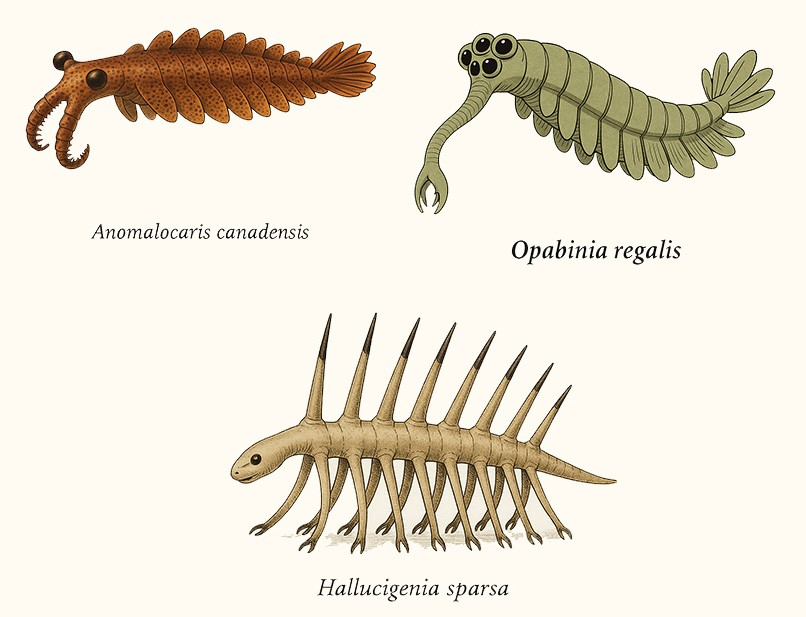
\includegraphics[width=0.5\textwidth]{images/cambriano_alieni.jpg}
    \caption{Le bizzarre creature del Cambriano: una ricostruzione di \textit{Anomalocaris}, \textit{Opabinia} e \textit{Hallucigenia}. Da questi primi esperimenti evolutivi, simili a creature lovecraftiane, sono emersi i primi e più semplici sistemi nervosi.}
    \label{fig:creature_cambriane}
\end{figure}

Immergiamoci nelle acque torbide del Cambriano, 550 milioni di anni fa. Qui nuotano creature che sembrano uscite da un incubo di H.P. Lovecraft: \textit{Anomalocaris} con i suoi occhi composti, \textit{Opabinia} con le sue cinque protuberanze oculari, \textit{Hallucigenia} che per decenni i paleontologi hanno ricostruito sottosopra\footnote{Morris, S. C., \& Caron, J. B. (2012). ``Pikaia gracilens Walcott, a stem-group chordate from the Middle Cambrian of British Columbia''. \textit{Biological Reviews}, 87(2), 480-512.}.

\begin{figure}[H]
    \centering
    
\includegraphics[width=0.8\textwidth]{evoluzione_cervello.png}
    \caption{Stratificazione evolutiva del cervello umano: 500 milioni di anni di bricolage neurologico}
    \label{fig:evoluzione_cervello}
\end{figure}

In questo teatro dell'assurdo evolutivo emerge la prima versione di quello che diventerà il nostro sistema nervoso. Non chiamatelo cervello: è più simile a un interruttore biologico con due sole posizioni: ``mangia'' o ``scappa''. 

Eppure, in questa semplicità brutale c'è già il seme di tutti i nostri futuri bias. Il proto-neurone che urlava ``pericolo!'' al minimo stimolo ambiguo è l'antenato diretto dell'amigdala\footnote{\textit{L'amigdala è una piccola struttura del cervello, situata nei lobi temporali, che funziona come centro di elaborazione delle emozioni (soprattutto paura e ansia) e della memoria emotiva.}} che oggi vi fa sobbalzare quando il tostapane espelle il pane. La differenza? Allora chi non sobbalzava finiva digerito. Oggi finite solo con il caffè rovesciato.

Questi primi neuroni cambriani ci insegnano una lezione fondamentale: già allora, la sopravvivenza non dipendeva dalla correttezza, ma dalla velocità. Era essenziale saper processare informazioni incomplete e decidere in fretta, anche a costo di sbagliare. Il trilobite che si fermava a riflettere se quella sagoma fosse un predatore o un'alga, non lasciava discendenti. Questa tendenza a favore dell'azione rapida basata su dati parziali – quella che oggi chiamiamo "saltare alle conclusioni" – è letteralmente codificata nei nostri circuiti neurali da oltre mezzo miliardo di anni.

\section{L'architettura stratificata: il modello del cervello trino}

Ora facciamo un salto in avanti di 150 milioni di anni. I vertebrati conquistano la terraferma e scoprono che l'aria è un pessimo conduttore di vibrazioni rispetto all'acqua. Improvvisamente, i predatori possono avvicinarsi in silenzio. La risposta evolutiva? Un potenziamento massiccio dei sistemi di allerta\footnote{Northcutt, R. G. (2002). ``Understanding vertebrate brain evolution''. \textit{Integrative and Comparative Biology}, 42(4), 743-756.}.

\index[main]{MacLean, Paul}Paul MacLean propose negli anni '60 il modello del ``\index[main]{cervello trino}cervello trino''\footnote{MacLean, P. D. (1990). \textit{The Triune Brain in Evolution: Role in Paleocerebral Functions}. New York: Plenum Press. Sebbene questo modello sia stato superato dalle neuroscienze moderne, rimane una metafora utile per comprendere la stratificazione evolutiva del cervello.}. Immaginate un grattacielo costruito sopra un castello medievale, a sua volta edificato su fondamenta romane. Ogni piano ha le sue regole architettoniche, i suoi sistemi di sicurezza, la sua logica interna. Al piano terra vive un guardiano paranoico di epoca preistorica, al primo piano abita un passionale conte medievale, e all'attico lavora un brillante scienziato moderno. Il problema sorge quando l'inquilino del piano terra --- il \index[main]{cervello rettiliano}cervello rettiliano --- decide che c'è un'emergenza e attiva l'allarme generale, mandando in tilt gli uffici moderni ai piani superiori.

\begin{figure}[h]
\centering

\includegraphics[width=0.8\textwidth]{cap1_1_condominio.png}
\caption{L'\index[main]{architettura cerebrale}Architettura Cerebrale Stratificata: come diverse ere evolutive convivono e comunicano nel nostro cervello}
\label{fig:brain_building}
\end{figure}

Questa \index[main]{architettura stratificata}architettura stratificata non è un caso di cattiva pianificazione. È il risultato di quello che \index[main]{Jacob, François}François Jacob chiamava ``\index[main]{bricolage evolutivo}bricolage evolutivo''\footnote{Jacob, F. (1977). ``Evolution and tinkering''. \textit{Science}, 196(4295), 1161-1166.}. L'evoluzione non può permettersi il lusso di riprogettare da zero: deve lavorare con quello che ha, modificando, adattando, riciclando strutture esistenti per nuovi scopi. Come ha osservato \index[main]{Dawkins, Richard}Richard Dawkins, ``l'evoluzione non ha \index[main]{preveggenza evolutiva}preveggenza''\footnote{Dawkins, R. (1986). \textit{The Blind Watchmaker}. New York: Norton.} --- può solo rispondere a \index[main]{pressioni selettive}pressioni selettive immediate, non pianificare per contingenze future.

Sebbene questa metafora sia stata superata dalle neuroscienze moderne, rimane un'utile semplificazione\footnote{Ruggiero, G. M., Ferro, M., Caselli, G., \& Sassaroli, S. (2022). ``Il cervello rettiliano esiste? CBT e cervello trino''. \textit{State of Mind}, 27 ottobre 2022.}. Oggi sappiamo infatti che il cervello non funziona come tre compartimenti stagni sovrapposti, ma piuttosto come una rete complessa di sistemi interconnessi e plastici\footnote{La ricerca moderna sui network cerebrali ha dimostrato che le funzioni cognitive emergono dall'interazione dinamica di reti distribuite piuttosto che da strutture isolate}.

Tuttavia, le funzioni che MacLean attribuiva a questi ``livelli'' esistono davvero – semplicemente non sono organizzate come pensava lui. Esistono davvero circuiti neurali che gestiscono:

\begin{itemize}
\item \textbf{Territorialità}: Da ``questo è il mio scoglio'' a ``questo è il mio parcheggio''
\item \textbf{Dominanza}: Da ``sono il maschio alfa'' a ``ho più follower su Instagram''
\item \textbf{Rituali}: Da ``danza di corteggiamento'' a ``routine mattutina del caffè''
\item \textbf{Aggressività}: Da ``mordo chi mi minaccia'' a ``flame war su Twitter''
\end{itemize}

Questi non sono comportamenti che abbiamo superato. Sono comportamenti che abbiamo sofisticato. Il manager che marca il territorio con oggetti personali in ufficio sta eseguendo lo stesso programma del varano che spruzza feromoni sul suo territorio.

\section{Il Prezzo della Coscienza: Perché Pensare Costa Caro}

Ogni ``difetto'' del nostro \index[main]{cervello}cervello è, in realtà, una cicatrice di guerra che testimonia una vittoria evolutiva. Ogni \index[main]{bias cognitivi}bias cognitivo è una scorciatoia che i nostri antenati hanno pagato a caro prezzo in termini di \index[main]{costo metabolico}costo metabolico. Il \index[main]{cervello umano}cervello umano, pur rappresentando solo il 2\% del peso corporeo, è un organo famelico: consuma circa il 20\% della nostra \index[main]{energia totale}energia totale\footnote{Raichle, M. E., \& Gusnard, D. A. (2002). ``Appraising the brain's energy budget''. \textit{Proceedings of the National Academy of Sciences}, 99(16), 10237-10239.}. In un mondo di scarsità calorica, ogni processo mentale doveva giustificare il suo dispendio energetico.

Questo spiega perché l'evoluzione non ci ha dato un cervello ``migliore'' e perfettamente razionale. Un sistema capace di \index[main]{analisi probabilistiche}analisi probabilistiche accurate in tempo reale sarebbe un lusso energetico insostenibile, come montare un motore di Formula 1 su una Fiat 500. L'evoluzione ha quindi preferito l'\index[main]{efficienza brutale}efficienza brutale alla perfezione analitica. Ha creato i ``bias'': \index[main]{scorciatoie cognitive}scorciatoie cognitive che ci permettono di prendere decisioni ``abbastanza buone'' consumando una frazione dell'energia.

\begin{figure}[h]
\centering
\textit{[Inserire qui: Infografica che confronta il peso del cervello (2\%) con il suo consumo energetico (20\%), mostrando il \index[main]{paradosso metabolico}paradosso metabolico che ha vincolato l'evoluzione cerebrale]}
\caption{Il Paradosso Energetico: come il vincolo metabolico ha plasmato la nostra \index[main]{architettura cognitiva}architettura cognitiva}
\label{fig:paradosso_energetico}
\end{figure}

Prendiamo l'\index[cognitive]{aracnofobia}aracnofobia. In Europa, la probabilità di morire per il morso di un ragno è statisticamente quasi nulla\footnote{Diaz, J. H. (2004). ``The global epidemiology, syndromic classification, management, and prevention of spider bites''. \textit{The American Journal of Tropical Medicine and Hygiene}, 71(2), 239-250.}. Eppure, la paura dei ragni è diffusa e potente. Dal punto di vista moderno, è irrazionale. Da quello evolutivo, è geniale. L'antenato che scattava al minimo sospetto di otto zampe aveva più probabilità di sopravvivere dell'antenato che si fermava a riflettere. Il costo di un \index[main]{falso positivo}falso positivo (scappare da un ragno innocuo) era minimo; il costo di un \index[main]{falso negativo}falso negativo (ignorare l'unico ragno velenoso) era fatale. L'evoluzione ha fatto i conti: meglio mille paure inutili che una singola morte evitabile.

\section{La rivoluzione mammifera: quando i bias divennero emotivi}

Circa 200 milioni di anni fa accade qualcosa di straordinario: l'evoluzione inventa le emozioni. Non le semplici reazioni stimolo-risposta dei rettili, ma esperienze soggettive complesse che colorano ogni percezione e decisione\footnote{Panksepp, J., \& Biven, L. (2012). \textit{The Archaeology of Mind: Neuroevolutionary Origins of Human Emotions}. Norton.}.

Il sistema limbico dei primi mammiferi introduce una novità rivoluzionaria: la capacità di ``sentire'' il futuro attraverso l'ansia e il passato attraverso il trauma. Se il cervello rettiliano viveva in un eterno presente di stimoli e risposte, quello mammaliano inizia a proiettare paure e speranze nel tempo.

Con l'avvento dei mammiferi, l'evoluzione introduce anche un'innovazione destinata a rivoluzionare il rapporto con la tecnologia: l'attaccamento sociale. I mammiferi, a differenza dei rettili che abbandonano le uova al loro destino, sviluppano legami emotivi profondi con la prole e, nelle specie più sociali, con il gruppo.

Questo sistema di attaccamento, mediato da neurotrasmettitori come l'ossitocina e la dopamina, è progettato per creare dipendenza: dipendenza dalla vicinanza fisica, dal contatto, dall'approvazione sociale. È un sistema così potente che può spingere un mammifero a sacrificare la propria vita per il gruppo.

Ora, spostate questo sistema nell'era digitale. Le notifiche dei social media, i ``like'', i messaggi, le email – tutti questi stimoli digitali attivano gli stessi circuiti neurali progettati per l'attaccamento mammifero. Il nostro cervello limbico non distingue tra l'approvazione fisica del branco e quella virtuale di Instagram. Il risultato? Una forma di attaccamento digitale che può essere altrettanto potente, e potenzialmente altrettanto problematica, dell'attaccamento fisico.

\section{Il grande balzo cognitivo: dalle reti primitive alle reti moderne}

L'ultima grande innovazione arriva con l'espansione della neocorteccia nei primati, culminando nell'ipertrofia che caratterizza \textit{Homo sapiens}. Per la prima volta, un animale può non solo reagire e sentire, ma anche \textit{riflettere} sulle proprie reazioni e sentimenti\footnote{Roth, G., \& Dicke, U. (2005). ``Evolution of the brain and intelligence''. \textit{Trends in Cognitive Sciences}, 9(5), 250-257.}.

Ma qui dobbiamo abbandonare definitivamente la metafora del ``cervello trino'' e abbracciare quello che le neuroscienze moderne ci hanno rivelato: il cervello umano non è un condominio con tre inquilini, ma una complessa orchestra di reti neurali interconnesse che suonano simultaneamente\footnote{Le neuroscienze moderne hanno identificato reti cerebrali dinamiche che cooperano e competono per guidare il comportamento e la cognizione}.

\section{Le tre reti che governano la nostra vita digitale}

La ricerca contemporanea ha identificato tre reti cerebrali fondamentali che determinano come reagiamo al mondo digitale\footnote{Il modello delle tre reti cerebrali (triple-network model) rappresenta il framework più accurato per comprendere le funzioni cognitive superiori}:

\subsection{La Default Mode Network (DMN): il narratore interiore}

La Default Mode Network è attiva quando non siamo impegnati in compiti esterni specifici, durante il mind-wandering, l'autoriflessione e la costruzione di narrative interne. Include regioni come il cortex prefrontale mediale, il cortex cingolato posteriore e il precuneo.

Questa rete è il nostro ``narratore interiore'' – quella voce mentale che commenta continuamente la nostra esperienza, crea connessioni tra eventi passati e futuri, e mantiene il senso di continuità del sé. È responsabile di quei momenti in cui, mentre scrollate Instagram, improvvisamente vi trovate a riflettere su una conversazione avuta tre anni fa o a immaginare scenari futuri basati su un post che avete appena visto.

\subsection{La Central Executive Network (CEN): il controllore di volo}

La Central Executive Network, anche chiamata Frontoparietal Network, è responsabile dell'attenzione focalizzata, del controllo esecutivo e della risoluzione di problemi complessi. Include principalmente la corteccia prefrontale dorsolaterale e il lobo parietale posteriore.

Questa è la nostra ``torre di controllo'' cognitiva – la rete che ci permette di mantenere l'attenzione su un compito, ignorare distrazioni, pianificare azioni complesse e monitorare le nostre prestazioni. È quella che dovrebbe impedirvi di controllare il telefono mentre state lavorando o leggendo questo libro.

\subsection{La Salience Network: l'interruttore dell'attenzione}

La Salience Network facilita lo switching tra le altre due reti, decidendo momento per momento se focalizzare l'attenzione verso l'interno (DMN) o verso compiti esterni (CEN). È centrata sull'insula anteriore e il cortex cingolato anteriore.

Questa rete è il nostro ``interruttore dell'attenzione'' – decide continuamente cosa merita la nostra attenzione e quando passare da un modo cognitivo all'altro. È quella che vi fa alzare lo sguardo dal libro quando sentite il vostro nome, o che vi fa notare una notifica del telefono anche quando siete concentrati su altro.

\begin{figure}[htbp]
    \centering
    \includegraphics[width=0.8\textwidth]{brain_networks.png}
    \caption{Le tre reti cerebrali nell'era digitale: un'orchestra senza direttore}
    \label{fig:brain_networks}
\end{figure}

\section{L'Agguato Digitale: Benvenuti nell'Era dell'Hacking Cognitivo}

Nel mondo digitale, i \index[main]{vincoli metabolici}vincoli metabolici che hanno forgiato i nostri bias vengono sfruttati contro di noi. Il \index[main]{multitasking}multitasking, considerato un'abilità moderna, è in realtà una violazione diretta della nostra \index[main]{architettura cognitiva ancestrale}architettura cognitiva ancestrale. Il cervello è ottimizzato per un'\index[main]{attenzione focalizzata}attenzione focalizzata e seriale. Quando tentiamo di gestire email, messaggi e chiamate simultaneamente, non stiamo facendo multitasking: stiamo costringendo il cervello a rapidi e costosi \index[main]{switch attentivi}switch attentivi, bruciando enormi quantità di \index[main]{glucosio}glucosio\footnote{Rubinstein, J. S., Meyer, D. E., \& Evans, J. E. (2001). ``Executive control of cognitive processes in task switching''. \textit{Journal of Experimental Psychology}, 130(4), 763.}. L'\index[main]{attenzione frammentata}attenzione frammentata è una forma di \index[main]{inefficienza metabolica}inefficienza metabolica senza precedenti.

Ma c'è di più. Le \index[main]{aziende tecnologiche}aziende tecnologiche hanno capito che i nostri bias non sono bug casuali, ma funzionalità prevedibili e hackerabili. Ogni app nel telefono è stata progettata da team di \index[main]{neuroscienziati}neuroscienziati, \index[main]{psicologi comportamentali}psicologi comportamentali e \index[main]{data scientist}data scientist per attivare i nostri meccanismi ancestrali. \index[main]{Instagram}Instagram ci mostra cibo e status sociale per attivare i \index[main]{circuiti neurali}circuiti neurali della ricompensa. \index[main]{TikTok}TikTok ha perfezionato l'arte del \index[main]{rinforzo intermittente}rinforzo intermittente, lo stesso principio che rende le \index[main]{slot machine}slot machine così assuefacenti: ricompense a intervalli imprevedibili che rendono il cervello dipendente dallo \index[main]{swipe}swipe successivo.

\begin{figure}[h]
\centering
\textit{[Inserire qui: Schema che mostra come diverse app sfruttano specifici bias cognitivi --- \index[main]{notifiche rosse}notifiche rosse (allerta pericolo), \index[main]{like}like (ricompense sociali), \index[main]{scroll infinito}scroll infinito (foraggiamento), \index[main]{streak}streak (paura di perdere status)]}
\caption{L'Anatomia dell'\index[main]{hacking cognitivo}Hacking Cognitivo: come le piattaforme digitali interfacciano con i nostri \index[main]{istinti ancestrali}istinti ancestrali}
\label{fig:hacking_cognitivo}
\end{figure}

È una forma inedita di \index[main]{jujitsu cognitivo}jujitsu cognitivo: per la prima volta nella storia, sistemi di \index[main]{intelligenza artificiale}intelligenza artificiale sfruttano in tempo reale le nostre vulnerabilità mentali più antiche. Se dovessimo ridurre la \index[main]{strategia evolutiva}strategia evolutiva del nostro cervello a uno \index[main]{pseudo-codice ancestrale}pseudo-codice ancestrale, sarebbe così:

\begin{verbatim}
SE (stimolo è minaccia potenziale) ALLORA
    Reagisci subito
    Razionalizza dopo (se sopravvivi)
ALTRIMENTI SE (stimolo è risorsa potenziale) ALLORA
    Afferra subito
    Valuta conseguenze dopo
ALTRIMENTI
    Risparmia energia
FINE SE
\end{verbatim}

Questo programma ancestrale è ancora il \index[main]{sistema operativo}sistema operativo di base del nostro comportamento. La nostra mente moderna può aggiungere livelli di complessità, ma sotto stress, torniamo sempre al codice originale.

Oggi, questo stesso ``principio del rilevatore di fumo'' si applica al nostro rapporto con la \index[main]{tecnologia digitale}tecnologia digitale. Il \index[cognitive]{bias di negatività}bias di negatività – la nostra tendenza a dare più peso alle informazioni negative – era vitale nella savana. Sui social media, dove gli algoritmi amplificano i contenuti che generano \index[main]{engagement emotivo}engagement emotivo, questo stesso bias ci tiene incollati a \index[main]{feed infiniti}feed infiniti di notizie allarmanti e polemiche. Non \index[main]{scrolling compulsivo}scrolliamo compulsivamente perché ci piaccia, ma perché il nostro \index[main]{cervello ancestrale}cervello ancestrale interpreta ogni titolo provocatorio come un potenziale pericolo da monitorare.

\section{Dalle rivoluzioni umane alla rivoluzione digitale}

Yuval Noah Harari, in Sapiens, identifica tre rivoluzioni che hanno progressivamente allontanato l'umanità dal suo contesto evolutivo originale:
"Circa 70.000 anni fa, la Rivoluzione Cognitiva diede inizio alla storia. Circa 12.000 anni fa, la Rivoluzione Agricola la accelerò. La Rivoluzione Scientifica, iniziata solo 500 anni fa, potrebbe porvi fine e dare inizio a qualcosa di completamente diverso."\footnote{Yuval Noah Harari, \textit{Sapiens: A Brief History of Humankind} (London: Harvill Secker, 2014), 3.}

Nel suo libro più recente, Nexus, Harari completa questo quadro identificando una quarta rivoluzione: la Rivoluzione dell'Intelligenza Artificiale\footnote{Yuval Noah Harari, \textit{Nexus: A Brief History of Information Networks from the Stone Age to AI} (New York: Random House, 2024), 15-30.}. Ciò che rende questa analisi particolarmente illuminante è come ognuna di queste rivoluzioni abbia aumentato esponenzialmente il disallineamento tra i nostri circuiti neurali e l'ambiente in cui viviamo.

\begin{figure}[htbp]
    \centering
    
\includegraphics[width=0.8\textwidth]{rivoluzioni.png}
    \caption{Accelerazione delle rivoluzioni umane secondo Harari (2014, 2024). La compressione temporale evidenzia il crescente disallineamento tra evoluzione biologica e cambiamento tecnologico.}
    \label{fig:rivoluzioni}
\end{figure}

Questa quarta rivoluzione rappresenta un salto qualitativo: mentre le precedenti hanno potenziato le capacità umane, l'AI potrebbe sostituire completamente il processo decisionale umano. Come osserva Harari, "l'AI non è uno strumento nelle nostre mani. L'AI è un agente indipendente che può sfuggire al nostro controllo, e noi possiamo diventare uno strumento nelle sue mani."\footnote{Ibid., 78.}

Il nostro cervello, che ha impiegato milioni di anni per sviluppare queste tre reti neurali sofisticate, ha avuto 12.000 anni per adattarsi parzialmente all'agricoltura, 500 anni per confrontarsi con la scienza, e solo 20 anni per gestire smartphone e social media. Ora deve confrontarsi con quella che Harari definisce "intelligenza aliena" - non extraterrestre, ma fondamentalmente diversa da quella umana nel modo in cui risolve problemi e persegue obiettivi\footnote{Ibid., 112-135.}.

\section{Un Difetto Provvidenziale: La Neurodiversità come Strategia Evolutiva}

C'è una tragica poesia in tutto questo. Abbiamo evoluto un cervello abbastanza sofisticato da riconoscere i propri limiti, ma non da superarli. Come osservava \index[main]{Pascal, Blaise}Pascal, ``l'uomo non è che una canna, la più fragile della natura; ma è una \index[main]{canna pensante}canna pensante''\footnote{Pascal, B. (1670). \textit{Pensées}. Sebbene Pascal non parlasse di bias cognitivi, la sua intuizione sulla natura paradossale della condizione umana rimane sorprendentemente attuale.}. Nell'era digitale, questa tragedia si amplifica: non solo siamo \index[main]{consapevolmente irrazionali}irrazionali, ma siamo costantemente manipolati da sistemi che conoscono la nostra irrazionalità meglio di noi.

E se queste \index[main]{distorsioni cognitive}distorsioni cognitive non fossero solo difetti, ma caratteristiche da gestire? E se la \index[main]{diversità cognitiva}diversità cognitiva fosse, essa stessa, una strategia evolutiva?\footnote{Nettle, D. (2006). ``The evolution of personality variation in humans and other animals''. \textit{American Psychologist}, 61(6), 622-631.} In un gruppo di \index[main]{cacciatori-raccoglitori}cacciatori-raccoglitori, avere profili psicologici diversi era un vantaggio. L'ansioso era la sentinella, il temerario l'esploratore. Questa \index[main]{neurodiversità funzionale}neurodiversità funzionale creava una forma di ``\index[main]{biodiversità cognitiva}biodiversità cognitiva'', rendendo il gruppo più resiliente.

\begin{figure}[h]
\centering
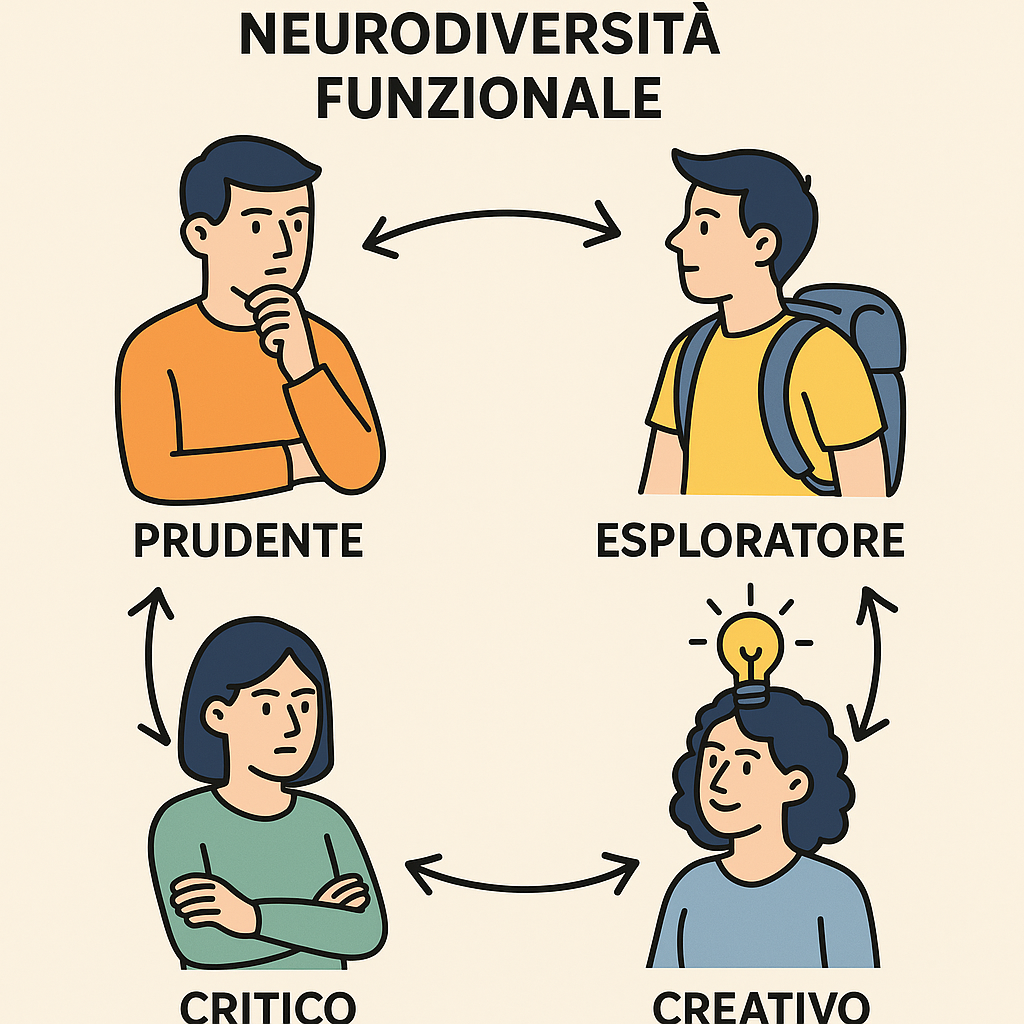
\includegraphics[width=0.8\textwidth]{images/neurodiversita.png}
\textit{[Inserire qui: Illustrazione di un gruppo con diversi profili cognitivi --- l'\index[main]{ansioso-sentinella}ansioso-sentinella, il \index[main]{temerario-esploratore}temerario-esploratore, il \index[main]{sospettoso-analitico}sospettoso-analitico, l'\index[main]{ottimista-motivatore}ottimista-motivatore --- che insieme creano un sistema resiliente]}
\caption{L'\index[main]{Orchestra Cognitiva}Orchestra Cognitiva: come la diversità dei bias individuali crea \index[main]{intelligenza collettiva}intelligenza collettiva adattiva}
\label{fig:orchestra_cognitiva}
\end{figure}

Questa prospettiva è cruciale oggi. Mentre l'IA tende all'\index[main]{ottimizzazione uniforme}ottimizzazione uniforme, la \index[main]{variabilità umana}variabilità umana è una risorsa strategica. Se tutti ragionassimo in modo ``perfetto'', saremmo vulnerabili agli stessi errori. La nostra ``\index[main]{irrazionalità distribuita}irrazionalità distribuita'' funziona come un \index[main]{ecosistema diversificato}ecosistema diversificato: meno efficiente nel breve termine, ma più robusto nel lungo periodo.

\section{L'illusione del controllo razionale}

Ma c'è una beffa evolutiva in tutto questo. L'espansione della neocorteccia ci ha dato non solo reti cognitive sofisticate, ma anche quello che Michael Gazzaniga chiama ``l'interprete del cervello sinistro''\footnote{Gazzaniga, M. S. (2000). ``Cerebral specialization and interhemispheric communication''. \textit{Brain}, 123(7), 1293-1326.}: un modulo dedicato a inventare spiegazioni razionali per decisioni prese da processi automatici e spesso inconsci.

È come avere un addetto stampa interno che deve costantemente giustificare le decisioni prese dalle diverse reti cerebrali. ``No, non ho passato tre ore su TikTok per procrastinare... stavo facendo ricerca sulla cultura giovanile contemporanea!''

La neocorteccia introduce capacità rivoluzionarie: pianificazione a lungo termine, pensiero astratto, linguaggio simbolico, capacità di immaginare scenari ipotetici. Ma introduce anche una maledizione: l'illusione del controllo razionale.

Questa illusione è particolarmente problematica nell'era digitale. La nostra CEN ci fa credere di essere noi a controllare le nostre scelte online, mentre in realtà stiamo reagendo a stimoli progettati per attivare automaticamente le nostre reti cerebrali più primitive. Pensiamo di scegliere razionalmente cosa guardare su Netflix, ma l'algoritmo sta giocando con i nostri circuiti della DMN e della Salience Network. Crediamo di decidere consciamente cosa comprare online, ma il sistema di raccomandazioni sta sfruttando i nostri bias di ancoraggio e disponibilità.

Ma l'illusione del controllo razionale nasconde un paradosso ancora più profondo, forse il più sconcertante di tutta la storia evolutiva.

\section{Il Paradosso Finale: La Fine della Selezione Naturale}

Per la prima volta in 3,5 miliardi di anni di vita sulla Terra, una specie ha raggiunto un punto in cui la \index[main]{selezione naturale}selezione naturale tradizionale si è sostanzialmente arrestata. Questa non è una conseguenza involontaria del progresso tecnologico: è il risultato diretto di quella stessa espansione neocorticale che ci ha dato l'illusione del controllo razionale.

Negli ultimi cento anni, il \index[main]{welfare tecnologico}welfare tecnologico e medico ha creato condizioni evolutive senza precedenti: la \index[main]{capacità riproduttiva}capacità riproduttiva non è più correlata ai vantaggi fisici, cognitivi o genetici tradizionali. Non importa più essere più forti, più intelligenti, più sani, o meglio adattati all'ambiente. L'unico parametro che determina il \index[main]{successo riproduttivo}successo riproduttivo è diventato puramente culturale: la \textit{voglia} di avere figli.

Questa è una \index[main]{rivoluzione silenziosa}rivoluzione silenziosa ma epocale. Per miliardi di anni, la riproduzione è stata il meccanismo attraverso cui l'evoluzione selezionava i tratti più adatti. Oggi, un genio della Silicon Valley con un QI di 180 e un patrimonio di miliardi può scegliere di non avere figli, mentre una famiglia senza particolari vantaggi genetici o economici può averne otto. Il \index[main]{successo evolutivo}successo evolutivo si è completamente svincolato dal \index[main]{successo adattivo}successo adattivo.

Non c'è più nessun vantaggio riproduttivo nell'essere più intelligenti, più forti, più sani, più alti, più belli. Sì, se sei più intelligente puoi avere statisticamente più successo economico, ma questo è totalmente disconnesso dall'avere figli. Puoi possedere tutti i vantaggi genetici immaginabili e scegliere di non riprodurrti. Puoi essere l'esatto opposto e avere una prole numerosa. L'\index[main]{unico parametro}unico parametro è ormai culturale: volere avere molti figli, completamente svincolato da qualsiasi caratteristica fisica o cognitiva.

Questo significa che il nostro corpo e il nostro cervello – questi capolavori di 500 milioni di anni di raffinamento evolutivo – potrebbero rappresentare simultaneamente l'apice e il punto finale dell'\index[main]{evoluzione biologica umana}evoluzione biologica umana. Non c'è più una direzione chiara verso cui la nostra specie si sta evolvendo fisicamente nei prossimi 100.000 anni. L'evoluzione continua, ma è diventata \index[main]{evoluzione culturale}culturale, non più biologica.

Il paradosso è sublime: proprio quando abbiamo raggiunto la sofisticazione cognitiva per comprendere e potenzialmente dirigere la nostra evoluzione, la selezione naturale ha smesso di dirigerla per noi. Siamo rimasti con \index[main]{cervelli paleolitici}cervelli paleolitici in corpi che non evolveranno più secondo le pressioni ambientali, ma che dovranno comunque navigare un futuro tecnologico in accelerazione costante.

È in questo contesto di \index[main]{stasi evolutiva biologica}stasi evolutiva biologica che dobbiamo inquadrare la sfida finale dell'era digitale.

\section{L'orchestrazione possibile}

La storia del nostro cervello culmina quindi in un paradosso: abbiamo evoluto reti neurali abbastanza sofisticate da comprendere la propria inadeguatezza per l'ambiente digitale, ma in un momento storico in cui l'evoluzione biologica non può più aiutarci ad adattarci. Siamo l'unica specie che può mappare i propri network cerebrali, studiare i propri limiti neurologici, e scrivere libri sulla propria natura conflittuale – eppure siamo anche l'unica specie che ha interrotto il processo evolutivo che ci ha portato a questa consapevolezza.

Ma forse stiamo interpretando male questa ``inadeguatezza''. La capacità di riconoscere i propri limiti non è una crudeltà evolutiva – è una caratteristica. Nessun'altra specie può dire: ``So che le mie reti cerebrali non sono ottimizzate per l'ambiente digitale, quindi creerò sistemi esterni per compensare questo disallineamento''. Nessun'altra specie può progettare tecnologie che amplifichino i punti di forza delle proprie reti neurali e mitighino le loro vulnerabilità.

Il sabotatore nella nostra testa, quindi, non è un nemico da sconfiggere. È un alleato tremendamente competente che lavora con una \index[main]{mappa obsoleta}mappa obsoleta. Non possiamo licenziarlo, né riprogrammarlo dopo 300.000 anni di esperienza e \index[main]{testardaggine evolutiva}testardaggine evolutiva. Possiamo però imparare a collaborare con lui. L'\index[main]{ansia}ansia è paralizzante davanti a Netflix, ma salvavita quando attraversiamo la strada. Il \index[cognitive]{bias di conferma}bias di conferma ci intrappola in \index[main]{bolle cognitive}bolle cognitive, ma ci dà la determinazione per finire progetti difficili.

La sfida per l'\index[main]{homo sapiens}homo sapiens del XXI secolo non è superare la propria natura – impresa impossibile e insensata. La sfida è imparare a navigare un mondo nuovo con \index[main]{strumenti cognitivi antichi}strumenti cognitivi antichi, riconoscendo quando ci aiutano e quando ci ostacolano. È diventare \index[main]{consapevolmente irrazionali}consapevolmente irrazionali.

Perché la lezione finale dell'evoluzione è questa: non siamo \index[main]{angeli della ragione}angeli della ragione caduti in un corpo animale. Siamo animali che hanno evoluto la straordinaria capacità di illudersi di essere angeli della ragione. E forse, in questa \index[main]{illusione necessaria}illusione necessaria, sta il segreto della nostra resilienza.

Ma come si fa a dirigere un'orchestra i cui strumenti sono stati forgiati in epoche diverse per scopi diversi? Bisogna iniziare conoscendo a fondo ogni singolo strumento, specialmente quelli più antichi e potenti, quelli il cui suono può sovrastare tutti gli altri.

E non c'è strumento più antico, potente e istintivo nel nostro repertorio mentale della paura. È il nostro sistema di allarme primordiale, un meccanismo essenziale che ci ha salvato la vita in innumerevoli occasioni. Nel prossimo capitolo, esploreremo come questo antico guardiano, un tempo indispensabile, reagisce al mondo moderno, trasformando spesso notifiche innocue in minacce esistenziali. Per imparare ad addomesticare gli algoritmi, dobbiamo prima capire come loro hanno imparato ad addomesticare le nostre paure.



%----------------------------------
% parte estratta dall versione finale del capitolo 1 da collocare da qualche altra parte>
\begin{comment}
E proprio questa mappa del conflitto interno, per quanto semplificata, è diventata l'oro della Silicon Valley. Mentre i neuroscienziati discutevano se il modello fosse anatomicamente corretto, gli ingegneri delle big tech avevano già capito l'essenziale: quando siamo stressati o emotivamente coinvolti, le parti primitive del cervello prendono il comando. Punto. Non importa quanto siamo intelligenti o istruiti -- sotto pressione, vinciamo sempre i circuiti più antichi.

%==================

\section{L'algoritmo ancestrale che governa ogni click}

Se dovessimo tradurre in codice il \index[main]{sistema operativo}sistema operativo del nostro cervello, scopriremmo qualcosa di imbarazzante nella sua semplicità. Trecento millenni di evoluzione umana si riducono a questo:

\begin{verbatim}
SE (stimolo = potenziale minaccia) ALLORA
    Reagisci immediatamente
    Pensa dopo (se sei ancora vivo)
ALTRIMENTI SE (stimolo = potenziale ricompensa) ALLORA
    Afferra subito
    Valuta conseguenze dopo (se necessario)
ALTRIMENTI
    Conserva energia
    Ignora
FINE SE
\end{verbatim}

Questo \index[main]{pseudo-codice ancestrale}pseudo-codice ancestrale non è una semplificazione didattica. È letteralmente come il nostro cervello prende decisioni quando non ha tempo di consultare la neocorteccia. E il bello -- o il tragico -- è che per il cervello "non avere tempo" significa qualsiasi situazione in cui c'è un minimo di stress emotivo, che oggi è praticamente sempre.

Il codice ha senso dal punto di vista evolutivo. Chi si fermava a filosofeggiare sul fruscio nell'erba veniva mangiato. Chi afferrava il frutto maturo senza indugio mangiava. Chi sprecava energia a processare stimoli irrilevanti moriva di fame. Semplice, brutale, efficace. Il problema è che questo stesso algoritmo ora deve processare derivati finanziari, relazioni poliamorose e abbonamenti a servizi streaming.

Ma ecco il colpo di genio -- o di perfidia, dipende dalle prospettive. Le \index[main]{aziende tecnologiche}aziende tecnologiche non hanno cercato di aggirare questo codice ancestrale. L'hanno abbracciato, studiato, ottimizzato. Hanno capito che non serviva convincere lo scienziato all'attico con argomenti razionali. Bastava parlare direttamente con il cavernicolo e il poeta, nella loro lingua primitiva fatta di colori, movimenti e ricompense immediate.

Prendiamo il \index[main]{design persuasivo}design persuasivo di qualsiasi app moderna. Non è un caso che le notifiche siano rosse. Il rosso, per il cavernicolo del piano terra, significa una cosa sola: sangue, pericolo, guarda immediatamente. Non importa che sia il 2025 e che il "pericolo" sia solo un commento su LinkedIn. Il cavernicolo vede rosso e attiva l'allarme generale. Lo scienziato all'attico può sapere benissimo che può aspettare, ma ormai l'adrenalina è in circolo.

I \index[main]{like}like e i cuoricini? È droga neurologica per il poeta del primo piano. Ogni piccolo cuore che appare sotto un post attiva lo stesso circuito di ricompensa che si accendeva quando la tribù ci accettava, quando il partner ci sceglieva, quando il gruppo ci riconosceva come membri. Solo che ora invece di succedere occasionalmente in situazioni sociali significative, succede centinaia di volte al giorno, creando una dipendenza da micro-validazioni che i nostri antenati non avrebbero potuto nemmeno immaginare.

E per lo scienziato razionale all'attico? Dashboard, analytics, percentuali di completamento, grafici colorati. "Eccoti i dati," sussurrano le app, "ora sei tu in controllo." Lo scienziato si sente appagato, convinto di star gestendo razionalmente il suo tempo digitale mentre consulta ossessivamente le statistiche di Screen Time, senza rendersi conto dell'ironia di controllare un'app per sapere quanto tempo passa sulle app.

Ma la strategia più diabolica è lo \index[main]{scroll infinito}scroll infinito. Questa è pura archeologia comportamentale applicata. Per milioni di anni, i nostri antenati hanno esplorato territori in cerca di risorse, sempre con la speranza che oltre la prossima collina ci fosse qualcosa di prezioso. Questo comportamento esplorativo è così profondamente cablato che non possiamo resistere. Il feed di Instagram o TikTok è progettato per sfruttare esattamente questo istinto: c'è sempre un altro post, un altro video, un'altra storia. Il prossimo potrebbe essere quello interessante, quello importante, quello che non puoi perdere.

\begin{center}
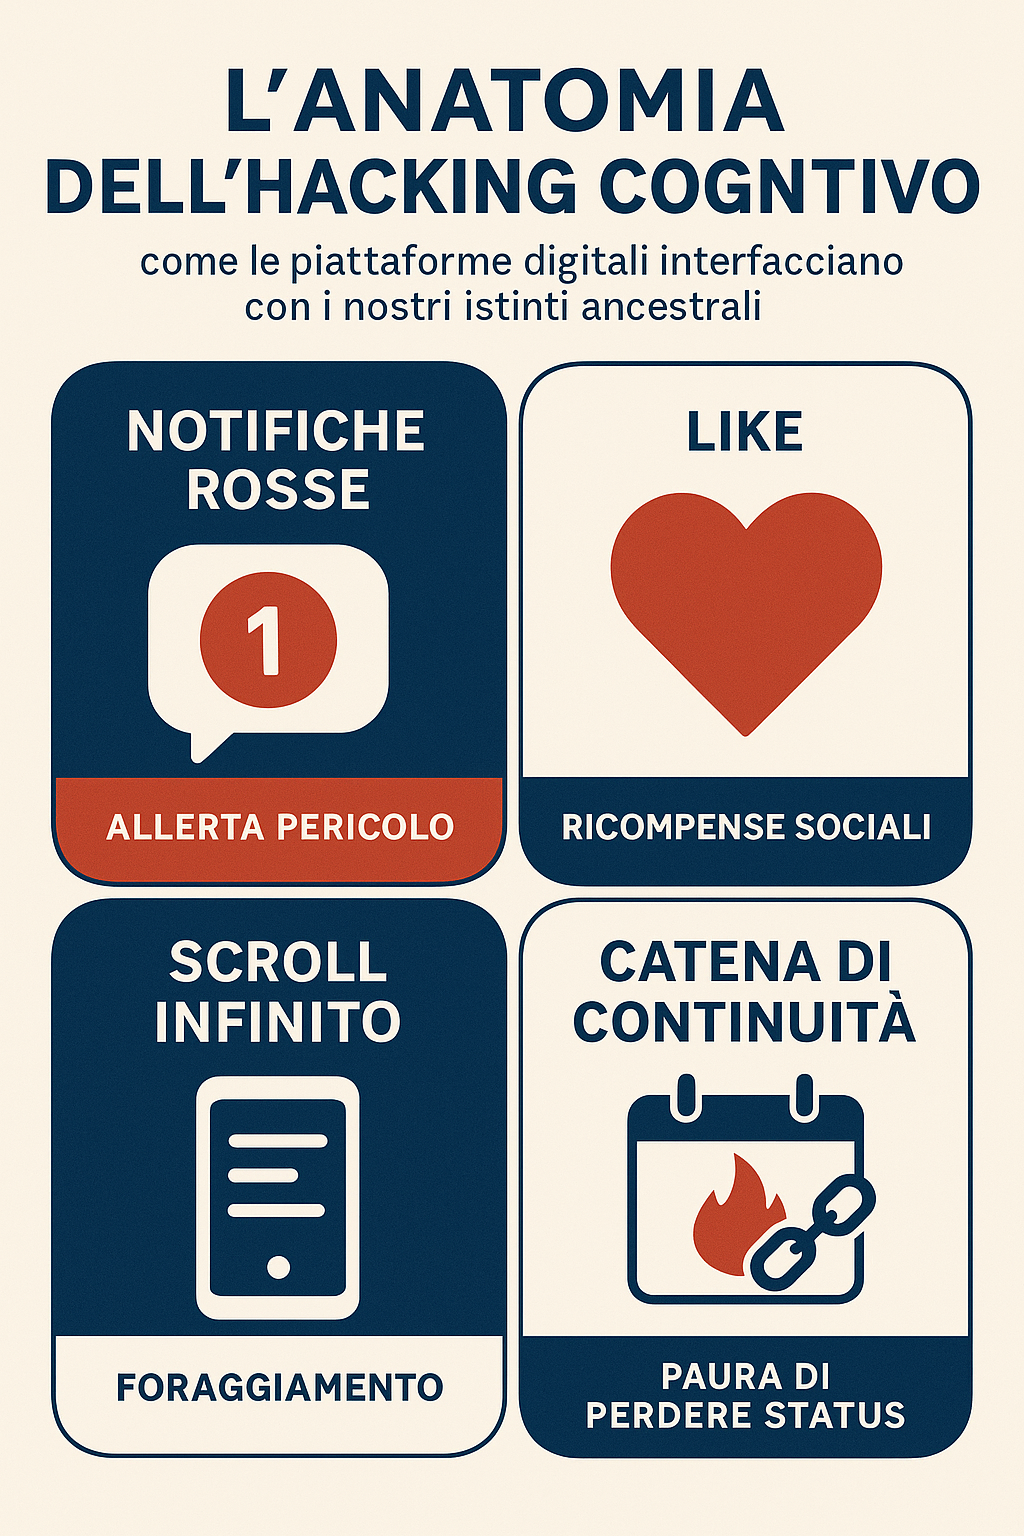
\includegraphics[width=0.5\textwidth]{images/hacking_cognitivo.png}
\captionof{figure}{L'\index[main]{hacking cognitivo}Anatomia dell'Hacking Cognitivo: come ogni elemento di design digitale parla a un diverso piano del nostro condominio cerebrale}
\label{fig:hacking_cognitivo}
\end{center}

Le \index[main]{catene di continuità}streak -- quelle serie di giorni consecutivi che molte app tracciano -- sono un capolavoro di manipolazione a tre livelli. Il cavernicolo vede la catena come territorio da difendere ("È mio! L'ho costruito!"). Il poeta la vive come una storia epica personale ("Sono al giorno 47 della mia saga!"). Lo scienziato la analizza come metrica di successo ("Sto ottimizzando la mia produttività!"). Risultato: vi sentite in colpa per rompere una serie di emoji fiammella su Snapchat come se aveste tradito un giuramento sacro.

C'è poi il sadismo sottile delle \index[main]{spunte blu}spunte blu e dei "visto". Prima del digitale, ignorare qualcuno richiedeva uno sforzo attivo: dovevi proprio girarti dall'altra parte. Ora, il sistema ti informa che il tuo messaggio è stato letto alle 15:47 e poi... silenzio. Il cavernicolo interpreta questo come ostracismo tribale. Il poeta ci ricama sopra tragedie degne di Racine. Lo scienziato calcola probabilità e formula ipotesi. Tutti e tre concordano: è una catastrofe sociale.

Il \index[main]{multitasking}multitasking è l'illusione suprema venduta alla nostra architettura cerebrale stratificata. Ci hanno convinto che possiamo gestire mail, Slack, WhatsApp, una call su Zoom e un podcast contemporaneamente. In realtà, quello che facciamo è \index[main]{task-switching}task-switching frenetico: il cervello salta da un contesto all'altro come un trapezista impazzito, bruciando glucosio come se stesse correndo una maratona\footnote{Rubinstein, J. S., Meyer, D. E., \& Evans, J. E. (2001). "Executive control of cognitive processes in task switching". \textit{Journal of Experimental Psychology}, 130(4), 763-797.}. 

Ma il costo non è solo metabolico. Ogni switch lascia quello che i neuroscienziati chiamano "residuo attentivo" -- parte della vostra mente rimane ancorata al task precedente. È come cercare di cambiare canale con un telecomando rotto che impiega 30 secondi a rispondere: quando finalmente cambia, avete già perso il filo di tutto.

La verità scomoda è che le aziende tecnologiche hanno psicologi comportamentali, neuroscienziati e data scientist che lavorano a tempo pieno per ottimizzare il loro dialogo con i vostri tre inquilini cerebrali. Ogni colore, ogni suono, ogni micro-animazione è testata su migliaia di cervelli per trovare la combinazione perfetta che massimizza l'engagement. È come se avessero le chiavi di casa vostra e potessero entrare quando vogliono, sussurrando al cavernicolo "Pericolo!", cantando serenate al poeta, mostrando grafici allo scienziato.

\section{L'inevitabilità magnifica del nostro destino neurologico}

 Il nostro cervello non è aggiornabile come un'app. Non possiamo fare un backup e installare Cervello OS 2.0 senza bug. Siamo bloccati con un'architettura neurologica progettata per problemi che non esistono più: distinguere bacche velenose, sfuggire ai predatori, mantenere lo status nella tribù di 150 individui. Oggi questi stessi circuiti devono decifrare clausole contrattuali, navigare dating app, e resistere all'algoritmo di TikTok.

Eppure -- e qui sta il miracolo -- siamo l'unica specie che può accorgersi di questo cortocircuito. Un piccione non sa di essere vittima del condizionamento operante quando becca ossessivamente una leva. Un cane non teorizza sui propri bias cognitivi. Solo noi possiamo osservare il nostro cervello mentre ci sabota e dire: "Ah, ecco cosa sta succedendo. Il cavernicolo ha preso il controllo."

Questa \index[main]{metacognizione}metacognizione -- la capacità di pensare al proprio pensiero -- è simultaneamente la nostra condanna e la nostra possibile redenzione. La condanna perché ci rende dolorosamente consapevoli di quanto siamo inadeguati al mondo che abbiamo creato. La redenzione perché è l'unico strumento che abbiamo per non essere completamente schiavi del nostro cablaggio ancestrale.

Non possiamo licenziare il cavernicolo paranoico del piano terra, né mandare in terapia il poeta melodrammatico del primo piano. Sono inquilini a vita nel nostro condominio mentale. Ma possiamo imparare a riconoscere quando hanno preso il controllo. Possiamo notare quando il cavernicolo scambia una notifica per un ruggito di leone. Possiamo accorgerci quando il poeta trasforma un "visualizzato" in tragedia greca. Possiamo sorridere quando lo scienziato crede di essere razionale mentre controlla compulsivamente le statistiche di produttività.

Il sabotatore nella vostra testa non è un nemico. È un sistema di navigazione progettato per le savane del Pleistocene che ora deve orientarsi in un labirinto digitale. Ha fatto un lavoro eccellente per 300.000 anni, tenendovi vivi abbastanza a lungo da riprodurvi. Il problema è che il mondo è cambiato più negli ultimi 20 anni che nei precedenti 20.000, e lui continua a navigare con mappe preistoriche.

Ma forse, proprio forse, capire questo è già metà della battaglia. Perché nel momento in cui riconoscete il cavernicolo, il poeta e lo scienziato dentro di voi, iniziate a vedere i fili che muovono la marionetta. E anche se non potete tagliare quei fili -- sono letteralmente i vostri neuroni -- almeno potete iniziare a capire chi li sta tirando e perché.

\bigskip

Ma c'è un inquilino del nostro condominio cerebrale che merita un'attenzione speciale. Uno che ha le chiavi di tutte le porte, può suonare l'allarme generale quando vuole, e lo fa con una frequenza imbarazzante nel mondo moderno. È il sistema più antico, più veloce e più potente che abbiamo: la paura.

Nel prossimo capitolo scenderemo nelle fondamenta del palazzo mentale, dove vive il più paranoico dei nostri inquilini. Scopriremo come un meccanismo progettato per salvarci dai leopardi nella savana oggi scatta per un messaggio visualizzato senza risposta. Esploreremo il paradosso di vivere nel periodo più sicuro della storia umana sentendoci costantemente in pericolo. E incontreremo i due piloti che guidano la nostra mente -- uno velocissimo ma miope, l'altro saggio ma sempre in ritardo -- in una corsa dove il primo ha sempre qualche metro di vantaggio.

Perché se il cervello trino ci ha mostrato l'architettura del conflitto, è la paura il carburante che alimenta la maggior parte dei nostri sabotaggi quotidiani. Ed è lì, in quel sistema d'allarme calibrato per un mondo che non esiste più, che si nasconde la chiave per capire perché facciamo quello che facciamo, anche quando sappiamo che non dovremmo farlo.

\end{comment}